%------------------------------------------------------------------------------
\section{Introduction}
Digital image processing underpins virtually every modern visual application---from
content-delivery networks resizing thumbnails for billions of users to medical
imaging pipelines analysing high-resolution scans. On CPUs, pixel-count growth
translates directly into latency: operating on a $7680{\times}4320$ (8K) image
requires 33 million pixels per pass, each demanding arithmetic on every pipeline
stage. GPUs break this bottleneck for \emph{data-parallel} tasks.
Operations such as Gaussian blurring, histogram equalization, and convolution
map naturally to CUDA's SIMT model and routinely achieve orders-of-magnitude
acceleration over single-threaded CPU~\cite{cudaguide}.

Content-aware image resizing, however, breaks the data-parallel assumption.
Seam carving~\cite{avidan2007} preserves salient image content while changing
dimensions by iteratively removing \emph{seams}---connected pixel paths of
least visual importance. Its dominant computation is a row-by-row dynamic
program (DP, Eq.~\eqref{eq:dp}) with an
\textbf{irreducible serial chain} of $H$ dependent steps: each row's result
depends strictly on the row above it, and no reordering eliminates this
dependency. Figure~\ref{fig:carve} shows the visual effect;
Figure~\ref{fig:dpstages} illustrates the DP.

Prior GPU implementations have taken three approaches, each with a cost.
Duarte and Sendag~\cite{duarte2012} kept one kernel launch per DP row,
achieving 231$\times$ on the energy kernel but leaving the serial DP as the
system bottleneck. Kiess~et~al.~\cite{kiess2014} used global-atomic
busy-waits for row synchronization in one persistent kernel, reaching
10.5$\times$ at the cost of warp occupancy.
Kim~et~al.~\cite{kim2015} sidestepped the DP entirely with a
non-cumulative heuristic reaching 76.6$\times$---trading exactness for
throughput, a reasonable choice when batches of seams are removed at once; their
own \emph{exact} single-block DP reached only 5.9$\times$ and was abandoned.

This paper asks a deliberately two-sided question: \emph{how fast can the exact
seam-carve DP run on a single V100, and---more importantly---what fundamentally
limits it?} The answer turns out to be the interesting part: after exhausting the
optimization space we reach only $6.2\times$ over a strong CPU, and we show this
ceiling is \emph{structural}, not a failure of engineering effort. Our
contributions are therefore as much a \emph{characterization of the limit} as an
optimization study:
(i) the optimization itself---\textbf{\emph{Tiled}}, which adapts the ghost-cell
stencil pattern with a seam-drift correctness bound to run $K{\approx}60$ column
strips without per-row global synchronization (the supporting single-block path
\textbf{\emph{Fused}}$\rightarrow$\textbf{\emph{Prefetch}}$\rightarrow$\textbf{\emph{BytePtr}},
guided by Nsight, contributes $1.7$--$2.1\times$ from latency hiding alone);
(ii) two impossibility arguments---the DP critical path is irreducible and a
transpose cannot reduce it;
(iii) a falsified escape---abandoning the DP for a greedy non-cumulative
selection gives \emph{no} speedup (${\approx}1.0\times$, Appendix~\ref{app:greedy}),
showing the DP is not even the end-to-end bottleneck;
(iv) the one lever that works---an approximate batch mode (amortize one pass over
$K$ seams) reaching $56\times$. Together these pin where the achievable frontier
of exact seam carving on a GPU actually lies, and why.

\begin{figure}[t]
  \centering
  \newlength{\carvefigh}\setlength{\carvefigh}{2.0cm}
  \begin{minipage}[b]{0.32\columnwidth}\centering
    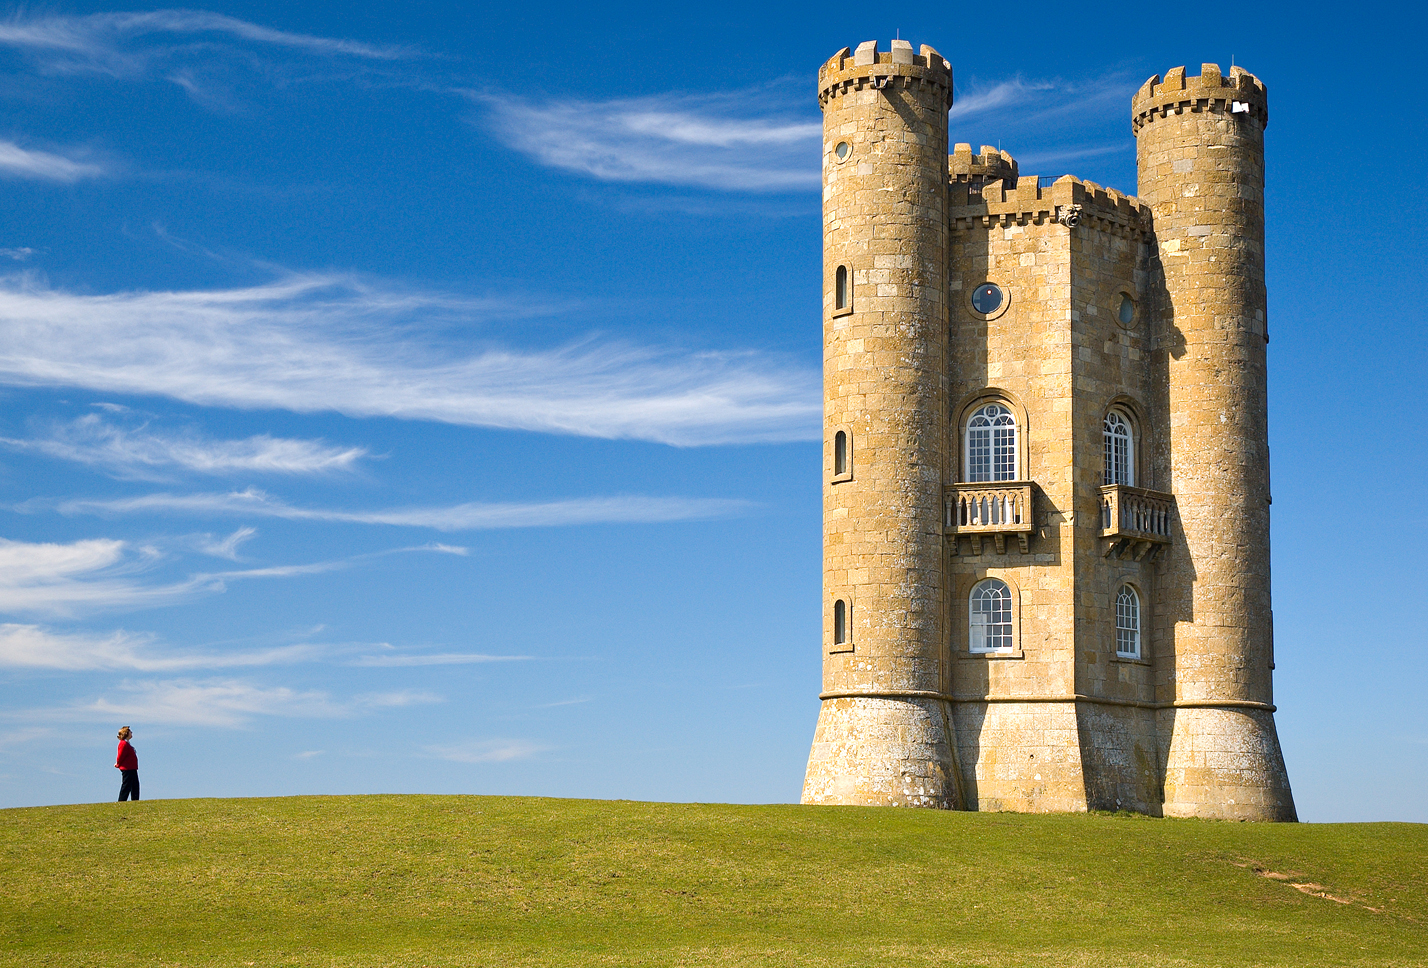
\includegraphics[height=\carvefigh,width=\linewidth,keepaspectratio]{figures/broadway_orig.jpg}\\[1pt]
    {\scriptsize (a) Original}
  \end{minipage}\hfill
  \begin{minipage}[b]{0.32\columnwidth}\centering
    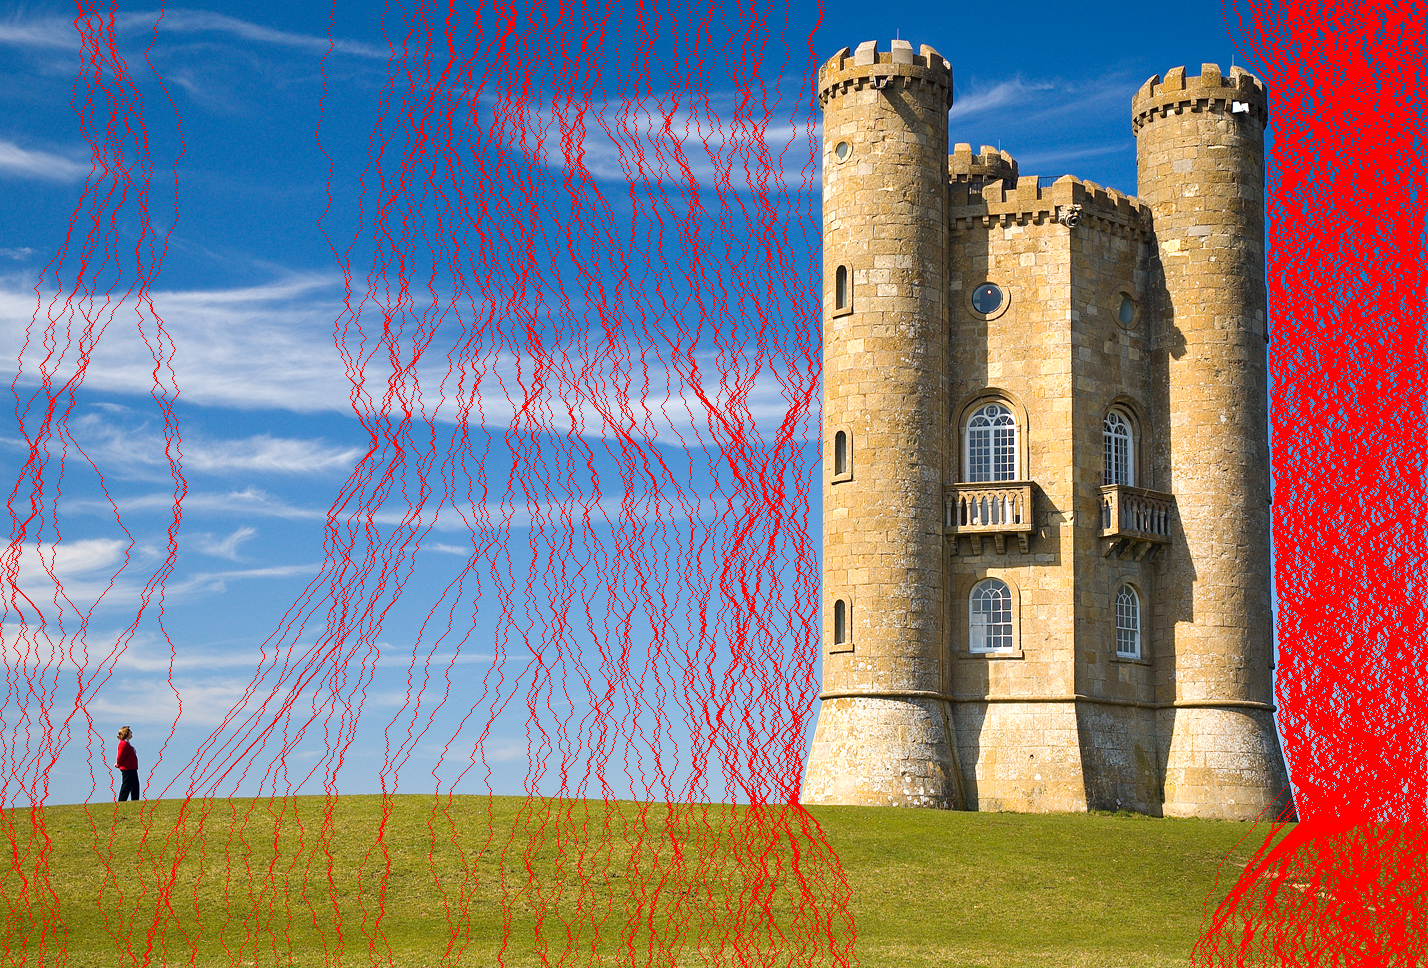
\includegraphics[height=\carvefigh,width=\linewidth,keepaspectratio]{figures/broadway_seams.png}\\[1pt]
    {\scriptsize (b) Seams (red)}
  \end{minipage}\hfill
  \begin{minipage}[b]{0.32\columnwidth}\centering
    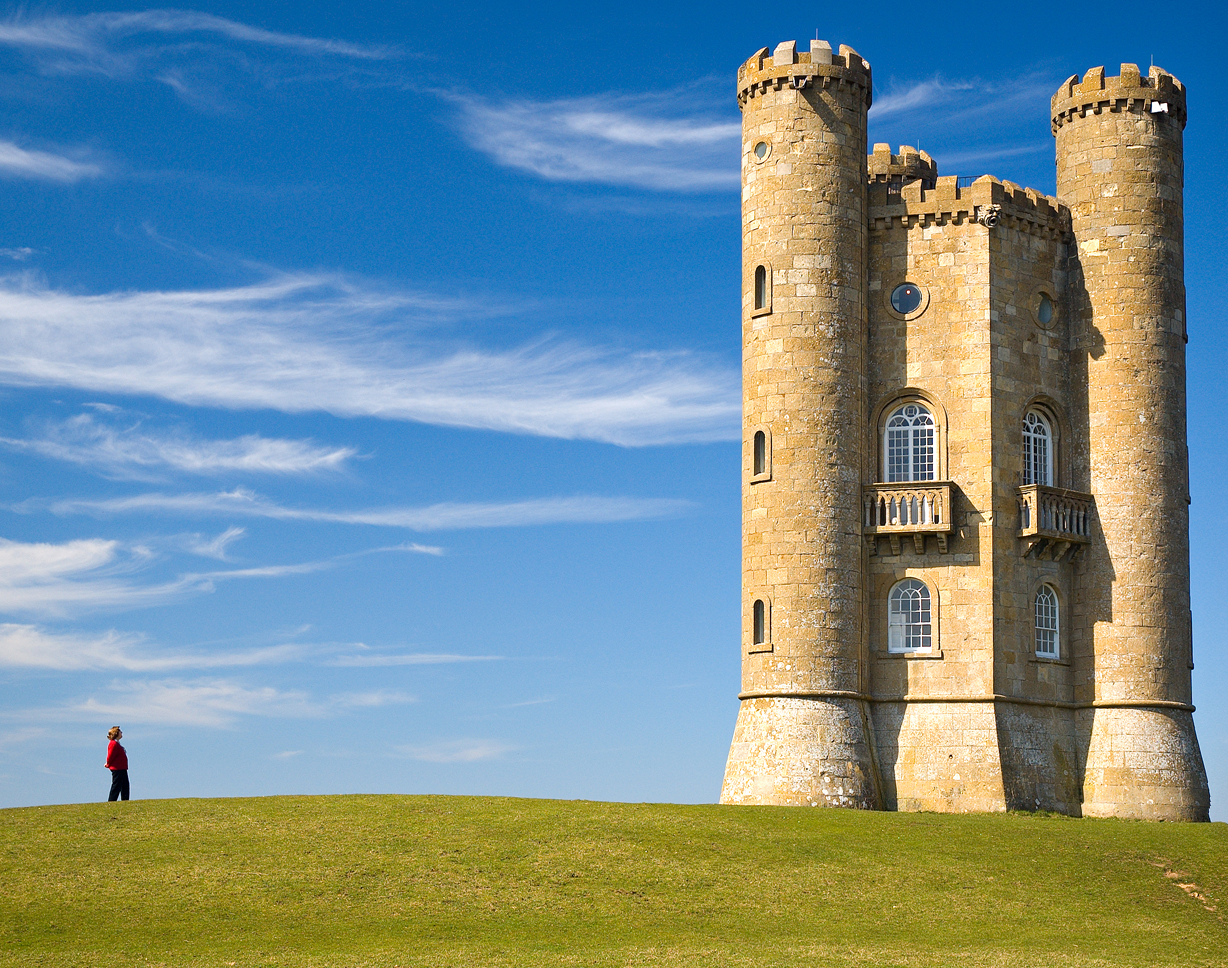
\includegraphics[height=\carvefigh,width=\linewidth,keepaspectratio]{figures/broadway_carved.png}\\[1pt]
    {\scriptsize (c) Carved}
  \end{minipage}
  \caption{Content-aware resizing: low-energy vertical seams (b) are removed
  iteratively, narrowing the image (c) while preserving salient structure.}
  \label{fig:carve}
\end{figure}
